\section{M{\o}ller Polarimeter}

\subsection{Physics Requirements and Polarimeter Design}

Several experiments in the proposed experimental program require the use of
polarized electron beams.  The design of the polarimeter for the upgrade is 
similar to the present polarimeter and will provide a similar uncertainty in 
the polarization measurement: $\Delta P_B/P_B\approx$2.5\%.

The polarimeter is based upon elastic electron-electron scattering.  The
electrons are detected in coincidence at center-of-mass scattering angles
near 90$^\circ$ where the analyzing power of the reaction, and therefore
the beam asymmetry, is a maximum.  For a beam of polarization $P_B^z$ and a
target of polarization $P_T^z$, the measured beam-helicity asymmetry is
given by:

\begin{equation}
\label{eq-Asym}
A=\frac{N_+-N_-}{N_++N_-}={\bar A}_{zz}P_B^zP_T^z,
\end{equation}

\noindent
where $N_+$ ($N_-$) is the number of counts with positive (negative) beam
helicity and ${\bar A}_{zz}$ is the average analyzing power for the beam 
and target polarized along the beam direction.  By detecting both of the 
scattered electrons over a small range of scattering angles, the reaction 
kinematics are fixed.  Thus, this method has the advantage, as compared to 
single-arm M{\o}ller polarimetry, of producing a clean data set without 
having to do energy-dependent background subtractions.  In the present 
{\tt CLAS} M{\o}ller polarimeter, accidental rates are typically less than 
5\% of the real rate for normal operating conditions.  Furthermore, the 
accidental rate is measured and included in the corrections.

The general layout of the present Hall B polarimeter is shown in
Fig.~\ref{fig-layout}.  It is located in the beamline immediately upstream
of the tagger. The system consists of a target chamber, two quadrupole
magnets, and two detectors in the horizontal plane on either side of the
beamline. The target is a permendur foil that is magnetized with a small
Helmholtz-coil system. The two quadrupoles separate the scattered electrons
from the unscattered beam. The two detectors are lead/scintillating fiber
composites. The magnets are powered by a power supply providing currents up
to 2676~A but is capable of providing 4800~A.

%%%%%%%%%%%%%%%%%%%%%%%%%%%%%%%%%%%%%%%%%%%%%%%%%%%%%%%%%%%%%%%%%%%%%%%%%
\begin{figure}[ht]
\centering
\includegraphics[width=12cm,angle=270]{layout.ps}
\caption{\small{Layout of the Hall B M{\o}ller polarimeter.}}
\label{fig-layout}
\end{figure}
%%%%%%%%%%%%%%%%%%%%%%%%%%%%%%%%%%%%%%%%%%%%%%%%%%%%%%%%%%%%%%%%%%%%%%%%%

The major components of the polarimeter -- target, magnets, detectors, and
power supply -- will be reused for 11~GeV operation, however, the relative
positioning of these elements will need to be modified and the
water-cooling system will need to be upgraded.  At a beam energy of 11~GeV,
the scattered electrons are not sufficiently deflected by the magnetic
field to reach the detectors in the present configuration.  Our simulations
indicate that running the power supply at the maximum current of 4800~A,
improves the situation.  At this current, the present cooling system cannot
handle the heat load, thus the need for an upgraded cooling system.

In addition, while the deflection angle of the scatted electrons increases
with the larger magnet currents, it is still not sufficient for the
electrons to be detected in the present configuration.  Simulations
indicate that this can be remedied by a combination of increasing the
flight path from the downstream quadrupole to the detectors, moving the
detectors closer to the beamline, and increasing the separation between the
quadrupoles. This will likely require moving both quadrupoles as well as
the target. More simulations are necessary to determine the geometrical 
configuration required for optimal operation.  We are thus planning for 
all three changes.

The changes to the geometrical configuration of the present polarimeter
will require several changes to the beamline and auxillary hardware.  This
includes new beam pipes, bellows, anchors, cables, and beam exit windows.

At 11~GeV a larger center-of-mass scattering-angle range will be
detected with the present detector system.  This reduces the effective
analyzing power of the polarimeter and thus increases measurement times
required to achieve the desired statistical precision.  Therefore, it will
be necessary to increase the segmentation of the detectors to restrict
and/or identify electrons in the desired angle range. This can be done
placing a smaller scintillator in front of each of the existing detectors.
These detectors would be half as wide and the same height as the present
detectors: 8~cm wide by 9~cm high.  This is preferable to simply reducing
the size of the present detectors, since the full present width is required
if polarization measurements are ever needed for beam energies in the range
of 5-8~GeV.

Finally, the existing polarimeter target system can be reused in its
present configuration.  However, since has been in use now since 1998, it
would be prudent to remeasure the target polarization, and if necessary,
replace the target material.  Replacement target material is in our
possession as well as the equipment to do the measurements.

\subsection{Collaboration and Responsibilities}

Florida International University is actively involved in this project. The
FIU nuclear physics group (5 faculty, 1 post doc, and 8 graduate students)
is currently supported by a DOE grant. The group's contribution to
{\tt CLAS12} will be the design of the polarimeter, construction of additional
detectors, and refurbishment of the target.  Design of the final polarimeter 
configuration will require further simulations to optimize performance. 
%Further simulations to determine the polarimeter's average analyzing power 
%will take place in 2008.  Construction of detectors and target refurbishment 
%are short lead-time items and are listed as being
%done in 2011 but can be done as late as 2012.


